% Data hierarchy of the eight datasets. Build: pdflatex datasets.tex && pdftoppm -png -r 200 -singlefile datasets.pdf datasets
\documentclass[tikz,border=8pt]{standalone}
\usepackage{amsmath,amssymb}
\usetikzlibrary{arrows.meta,calc}
\definecolor{cC}{HTML}{7B4FB8}\definecolor{cL}{HTML}{1C9A8A}
\tikzset{
  arr/.style={-{Stealth[length=2mm]},line width=0.6pt,draw=black!60},
  bundle/.style={draw=black!60,fill=black!10,line width=0.7pt,rounded corners=2pt,minimum width=3.9cm,minimum height=0.62cm,font=\small,align=center},
  item/.style={draw=black!60,fill=white,line width=0.7pt,rounded corners=2pt,minimum width=3.9cm,minimum height=0.62cm,font=\small,align=center},
  used/.style={draw=cL,fill=cL!14,line width=1pt,rounded corners=2pt,minimum width=3.9cm,minimum height=0.62cm,font=\small,align=center},
  textonly/.style={draw=cC,fill=cC!8,line width=0.7pt,dash pattern=on 3pt off 1.5pt,rounded corners=2pt,minimum width=3.9cm,minimum height=0.62cm,font=\small,align=center},
  unused/.style={draw=black!40,fill=white,line width=0.7pt,dash pattern=on 1.5pt off 1.5pt,rounded corners=2pt,minimum width=3.9cm,minimum height=0.62cm,font=\small,align=center,text=black!60},
  rel/.style={font=\scriptsize,text=black!55,fill=white,inner sep=1pt},
  stat/.style={font=\small,anchor=north west,align=left},
  note/.style={font=\scriptsize,text=black!55,align=left,anchor=north west},
  title/.style={font=\bfseries,anchor=west},
  frame/.style={draw=black!20,line width=0.6pt,rounded corners=6pt},
}
% \chain{x}{y}{style 1/text 1, style 2/text 2, ...}{relation labels}: boxes top-down from (x, y)
\newcommand{\chain}[4]{%
  \foreach \s/\t [count=\i] in {#3}{\node[\s] (b\i) at (#1,{#2-0.98*(\i-1)}) {\t};}
  \foreach \r [count=\i] in {#4}{\pgfmathtruncatemacro{\j}{\i+1}\draw[arr] (b\i) -- node[rel,right=1mm]{\r} (b\j);}}
% \panel{x}{y}{height}{title}
\newcommand{\panel}[4]{\draw[frame] (#1-0.3,#2+0.75) rectangle ++(9.4,-#3);\node[title] at (#1-0.1,#2+0.35) {#4};}

\begin{document}
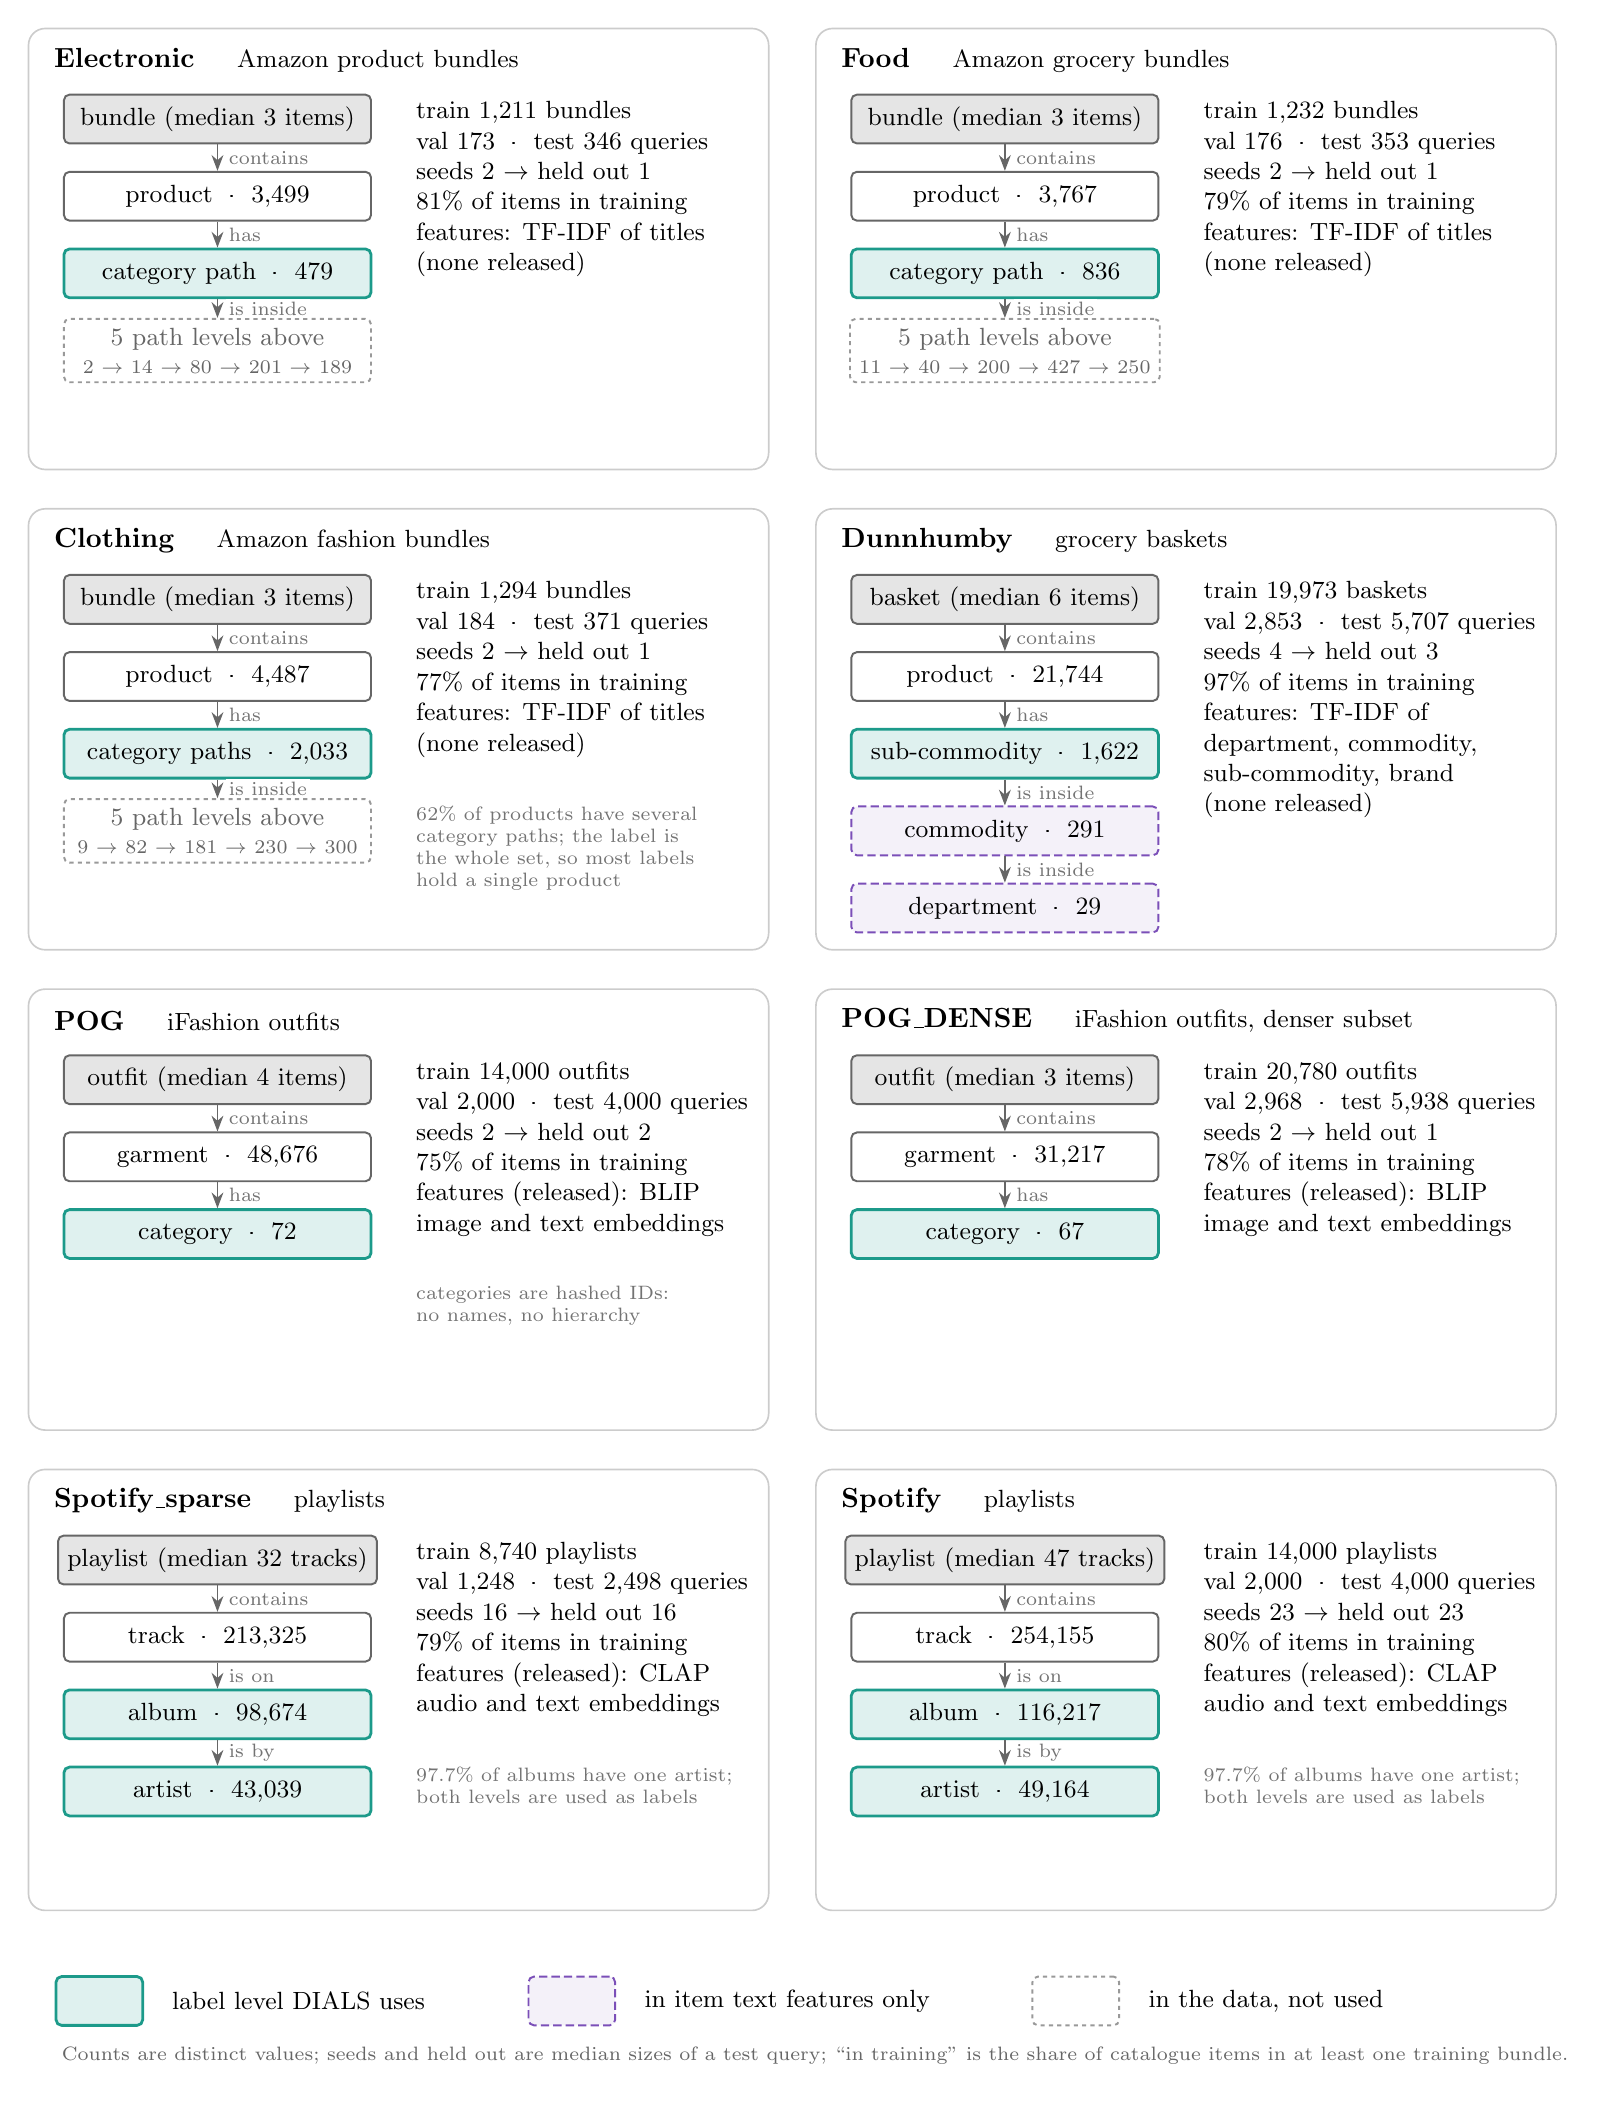
\begin{tikzpicture}[x=1cm,y=1cm]
\def\H{5.6}
% ---------------------------------------------------------------- row 1: e-commerce
\begin{scope}[shift={(0,0)}]
\panel{0}{0}{\H}{Electronic \quad\normalfont\small Amazon product bundles}
\chain{2.1}{-0.4}{bundle/bundle (median 3 items),item/product \;·\; 3{,}499,used/category path \;·\; 479,unused/5 path levels above\\[-1pt]{\scriptsize 2 $\to$ 14 $\to$ 80 $\to$ 201 $\to$ 189}}{contains,has,is inside}
\node[stat] at (4.5,-0.05) {train 1{,}211 bundles\\val 173 \;·\; test 346 queries\\seeds 2 $\to$ held out 1\\81\% of items in training\\features: TF-IDF of titles\\(none released)};
\end{scope}
\begin{scope}[shift={(10,0)}]
\panel{0}{0}{\H}{Food \quad\normalfont\small Amazon grocery bundles}
\chain{2.1}{-0.4}{bundle/bundle (median 3 items),item/product \;·\; 3{,}767,used/category path \;·\; 836,unused/5 path levels above\\[-1pt]{\scriptsize 11 $\to$ 40 $\to$ 200 $\to$ 427 $\to$ 250}}{contains,has,is inside}
\node[stat] at (4.5,-0.05) {train 1{,}232 bundles\\val 176 \;·\; test 353 queries\\seeds 2 $\to$ held out 1\\79\% of items in training\\features: TF-IDF of titles\\(none released)};
\end{scope}
% ---------------------------------------------------------------- row 2
\begin{scope}[shift={(0,-6.1)}]
\panel{0}{0}{\H}{Clothing \quad\normalfont\small Amazon fashion bundles}
\chain{2.1}{-0.4}{bundle/bundle (median 3 items),item/product \;·\; 4{,}487,used/category paths \;·\; 2{,}033,unused/5 path levels above\\[-1pt]{\scriptsize 9 $\to$ 82 $\to$ 181 $\to$ 230 $\to$ 300}}{contains,has,is inside}
\node[note] at (4.5,-2.9) {62\% of products have several\\category paths; the label is\\the whole set, so most labels\\hold a single product};
\node[stat] at (4.5,-0.05) {train 1{,}294 bundles\\val 184 \;·\; test 371 queries\\seeds 2 $\to$ held out 1\\77\% of items in training\\features: TF-IDF of titles\\(none released)};
\end{scope}
\begin{scope}[shift={(10,-6.1)}]
\panel{0}{0}{\H}{Dunnhumby \quad\normalfont\small grocery baskets}
\chain{2.1}{-0.4}{bundle/basket (median 6 items),item/product \;·\; 21{,}744,used/sub-commodity \;·\; 1{,}622,textonly/commodity \;·\; 291,textonly/department \;·\; 29}{contains,has,is inside,is inside}
\node[stat] at (4.5,-0.05) {train 19{,}973 baskets\\val 2{,}853 \;·\; test 5{,}707 queries\\seeds 4 $\to$ held out 3\\97\% of items in training\\features: TF-IDF of\\department, commodity,\\sub-commodity, brand\\(none released)};
\end{scope}
% ---------------------------------------------------------------- row 3: POG
\begin{scope}[shift={(0,-12.2)}]
\panel{0}{0}{\H}{POG \quad\normalfont\small iFashion outfits}
\chain{2.1}{-0.4}{bundle/outfit (median 4 items),item/garment \;·\; 48{,}676,used/category \;·\; 72}{contains,has}
\node[stat] at (4.5,-0.05) {train 14{,}000 outfits\\val 2{,}000 \;·\; test 4{,}000 queries\\seeds 2 $\to$ held out 2\\75\% of items in training\\features (released): BLIP\\image and text embeddings};
\node[note] at (4.5,-2.9) {categories are hashed IDs:\\no names, no hierarchy};
\end{scope}
\begin{scope}[shift={(10,-12.2)}]
\panel{0}{0}{\H}{POG\_DENSE \quad\normalfont\small iFashion outfits, denser subset}
\chain{2.1}{-0.4}{bundle/outfit (median 3 items),item/garment \;·\; 31{,}217,used/category \;·\; 67}{contains,has}
\node[stat] at (4.5,-0.05) {train 20{,}780 outfits\\val 2{,}968 \;·\; test 5{,}938 queries\\seeds 2 $\to$ held out 1\\78\% of items in training\\features (released): BLIP\\image and text embeddings};
\end{scope}
% ---------------------------------------------------------------- row 4: Spotify
\begin{scope}[shift={(0,-18.3)}]
\panel{0}{0}{\H}{Spotify\_sparse \quad\normalfont\small playlists}
\chain{2.1}{-0.4}{bundle/playlist (median 32 tracks),item/track \;·\; 213{,}325,used/album \;·\; 98{,}674,used/artist \;·\; 43{,}039}{contains,is on,is by}
\node[stat] at (4.5,-0.05) {train 8{,}740 playlists\\val 1{,}248 \;·\; test 2{,}498 queries\\seeds 16 $\to$ held out 16\\79\% of items in training\\features (released): CLAP\\audio and text embeddings};
\node[note] at (4.5,-2.9) {97.7\% of albums have one artist;\\both levels are used as labels};
\end{scope}
\begin{scope}[shift={(10,-18.3)}]
\panel{0}{0}{\H}{Spotify \quad\normalfont\small playlists}
\chain{2.1}{-0.4}{bundle/playlist (median 47 tracks),item/track \;·\; 254{,}155,used/album \;·\; 116{,}217,used/artist \;·\; 49{,}164}{contains,is on,is by}
\node[stat] at (4.5,-0.05) {train 14{,}000 playlists\\val 2{,}000 \;·\; test 4{,}000 queries\\seeds 23 $\to$ held out 23\\80\% of items in training\\features (released): CLAP\\audio and text embeddings};
\node[note] at (4.5,-2.9) {97.7\% of albums have one artist;\\both levels are used as labels};
\end{scope}
% ---------------------------------------------------------------- legend
\begin{scope}[shift={(0,-24.3)}]
\node[used,minimum width=1.1cm] at (0.6,0) {};\node[stat,anchor=west] at (1.4,0) {label level DIALS uses};
\node[textonly,minimum width=1.1cm] at (6.6,0) {};\node[stat,anchor=west] at (7.4,0) {in item text features only};
\node[unused,minimum width=1.1cm] at (13.0,0) {};\node[stat,anchor=west] at (13.8,0) {in the data, not used};
\node[stat,anchor=west,text=black!60,font=\scriptsize] at (0.0,-0.7) {Counts are distinct values; seeds and held out are median sizes of a test query; ``in training'' is the share of catalogue items in at least one training bundle.};
\end{scope}
\end{tikzpicture}
\end{document}
